% Version 1.2 of SN LaTeX, November 2022
%
% See section 11 of the User Manual for version history 
%
%%%%%%%%%%%%%%%%%%%%%%%%%%%%%%%%%%%%%%%%%%%%%%%%%%%%%%%%%%%%%%%%%%%%%%
%%                                                                 %%
%% Please do not use \input{...} to include other tex files.       %%
%% Submit your LaTeX manuscript as one .tex document.              %%
%%                                                                 %%
%% All additional figures and files should be attached             %%
%% separately and not embedded in the \TeX\ document itself.       %%
%%                                                                 %%
%%%%%%%%%%%%%%%%%%%%%%%%%%%%%%%%%%%%%%%%%%%%%%%%%%%%%%%%%%%%%%%%%%%%%

%%\documentclass[referee,sn-basic]{sn-jnl}% referee option is meant for double line spacing

%%=======================================================%%
%% to print line numbers in the margin use lineno option %%
%%=======================================================%%

%%\documentclass[lineno,sn-basic]{sn-jnl}% Basic Springer Nature Reference Style/Chemistry Reference Style

%%======================================================%%
%% to compile with pdflatex/xelatex use pdflatex option %%
%%======================================================%%

%%\documentclass[pdflatex,sn-basic]{sn-jnl}% Basic Springer Nature Reference Style/Chemistry Reference Style


%%Note: the following reference styles support Namedate and Numbered referencing. By default the style follows the most common style. To switch between the options you can add or remove “Numbered” in the optional parenthesis. 
%%The option is available for: sn-basic.bst, sn-vancouver.bst, sn-chicago.bst, sn-mathphys.bst. %  
 
%%\documentclass[sn-nature]{sn-jnl}% Style for submissions to Nature Portfolio journals
%%\documentclass[sn-basic]{sn-jnl}% Basic Springer Nature Reference Style/Chemistry Reference Style
\documentclass[sn-mathphys,Numbered]{sn-jnl}% Math and Physical Sciences Reference Style
%%\documentclass[sn-aps]{sn-jnl}% American Physical Society (APS) Reference Style
%%\documentclass[sn-vancouver,Numbered]{sn-jnl}% Vancouver Reference Style
%%\documentclass[sn-apa]{sn-jnl}% APA Reference Style 
%%\documentclass[sn-chicago]{sn-jnl}% Chicago-based Humanities Reference Style
%%\documentclass[default]{sn-jnl}% Default
%%\documentclass[default,iicol]{sn-jnl}% Default with double column layout

%%%% Standard Packages
%%<additional latex packages if required can be included here>

\usepackage{graphicx}%
\usepackage{multirow}%
\usepackage{amsmath,amssymb,amsfonts}%
\usepackage{amsthm}%
\usepackage{mathrsfs}%
\usepackage[title]{appendix}%
\usepackage{xcolor}%
\usepackage{textcomp}%
\usepackage{manyfoot}%
\usepackage{booktabs}%
\usepackage{algorithm}%
\usepackage{algorithmicx}%
\usepackage{algpseudocode}%
\usepackage{listings}%
\usepackage{indentfirst}%
%%%%

%%%%%=============================================================================%%%%
%%%%  Remarks: This template is provided to aid authors with the preparation
%%%%  of original research articles intended for submission to journals published 
%%%%  by Springer Nature. The guidance has been prepared in partnership with 
%%%%  production teams to conform to Springer Nature technical requirements. 
%%%%  Editorial and presentation requirements differ among journal portfolios and 
%%%%  research disciplines. You may find sections in this template are irrelevant 
%%%%  to your work and are empowered to omit any such section if allowed by the 
%%%%  journal you intend to submit to. The submission guidelines and policies 
%%%%  of the journal take precedence. A detailed User Manual is available in the 
%%%%  template package for technical guidance.
%%%%%=============================================================================%%%%

%\jyear{2021}%

%% as per the requirement new theorem styles can be included as shown below
\theoremstyle{thmstyleone}%
\newtheorem{theorem}{Theorem}%  meant for continuous numbers
%%\newtheorem{theorem}{Theorem}[section]% meant for sectionwise numbers
%% optional argument [theorem] produces theorem numbering sequence instead of independent numbers for Proposition
\newtheorem{proposition}[theorem]{Proposition}% 
%%\newtheorem{proposition}{Proposition}% to get separate numbers for theorem and proposition etc.

\theoremstyle{thmstyletwo}%
\newtheorem{example}{Example}%
\newtheorem{remark}{Remark}%

\theoremstyle{thmstylethree}%
\newtheorem{definition}{Definition}%

\raggedbottom
%%\unnumbered% uncomment this for unnumbered level heads

\begin{document}

\title[Article Title]{Prediction of tubing pressure based on Bi-LSTM neural structure with innovative forecasting strategy}


%%=============================================================%%
%% Prefix	-> \pfx{Dr}
%% GivenName	-> \fnm{Joergen W.}
%% Particle	-> \spfx{van der} -> surname prefix
%% FamilyName	-> \sur{Ploeg}
%% Suffix	-> \sfx{IV}
%% NatureName	-> \tanm{Poet Laureate} -> Title after name
%% Degrees	-> \dgr{MSc, PhD}
%% \author*[1,2]{\pfx{Dr} \fnm{Joergen W.} \spfx{van der} \sur{Ploeg} \sfx{IV} \tanm{Poet Laureate} 
%%                 \dgr{MSc, PhD}}\email{iauthor@gmail.com}
%%=============================================================%%

\author[1]{\fnm{Zikang} \sur{Zhong}}\email{zzk1637@outlook.com}

\author*[2]{\fnm{Jianjun} \sur{Zhu}}\email{jianjun-zhu@cup.edu.cn}

\author*[3]{\fnm{Jianli} \sur{Wang}}\email{wangjianli@seu.edu.cn}


\affil[1]{\orgdiv{Department of Mechanical Engineering}, \orgname{Southeast University}, \orgaddress{ \city{Nanjing}, \postcode{210096}, \country{China}}}

\affil[2]{\orgdiv{College of Mechanical and Transportation Engineering}, \orgname{China University of Petroleum}, \orgaddress{\city{Beijing}, \postcode{102249}, \country{China}}}

%%\affil[3]{\orgdiv{Department}, \orgname{Organization}, \orgaddress{\street{Street}, \city{City}, \postcode{610101}, \state{State}, \country{Country}}}

%%==================================%%
%% sample for unstructured abstract %%
%%==================================%%

\abstract{Plunger lift is commonly applied to both conventional and unconventional gas wells to tackle issues such as liquid loading, which can cause the liquid in gas wells loaded up and even cease production (Park et al., 2009; Paulo te al., 2015; Fadairo et al., 2015; Zhang et al., 2010). However, the overall system consists of moving parts and dynamic multiphase flow, which is complex and may suffer from production instability. With the machine learning (ML) algorithms, the well surveillance data can be harnessed to forecast the production rates of gas wells assisted by the plunger lift, which helps guide the decision-making of gas well deliquification. Several deep learning algorithms, e.g., RNN's (regular recurrent neural network), LSTM (long short-term memory)., have been proven to be able to capture the temporal dynamic behaviors of the time-series data. In this paper, a case study of the recurrent neural network based on LSTM for production data analytics was carried out. The model regression accuracies and computational efficiencies of different models were compared experimentally. The comparison shows that the encoder-decoder architecture combined with bidirectional LSTM (BILSTM-AE), multi-forecast average bidirectional LSTM (ABILSTM), and noise smooth bidirectional LSTM (SBILSTM) achieved the lowest error of RMSE (1.20\%, 1.09\%, and 0.95\%, respectively) and highest R2 scores (95.49\%, 96.97\%, and 96.38\%, respectively). A further statistical comparison reveals that the ABILSTM model demonstrates the most impressive performance among others.}

%%================================%%
%% Sample for structured abstract %%
%%================================%%

% \abstract{\textbf{Purpose:} The abstract serves both as a general introduction to the topic and as a brief, non-technical summary of the main results and their implications. The abstract must not include subheadings (unless expressly permitted in the journal's Instructions to Authors), equations or citations. As a guide the abstract should not exceed 200 words. Most journals do not set a hard limit however authors are advised to check the author instructions for the journal they are submitting to.
% 
% \textbf{Methods:} The abstract serves both as a general introduction to the topic and as a brief, non-technical summary of the main results and their implications. The abstract must not include subheadings (unless expressly permitted in the journal's Instructions to Authors), equations or citations. As a guide the abstract should not exceed 200 words. Most journals do not set a hard limit however authors are advised to check the author instructions for the journal they are submitting to.
% 
% \textbf{Results:} The abstract serves both as a general introduction to the topic and as a brief, non-technical summary of the main results and their implications. The abstract must not include subheadings (unless expressly permitted in the journal's Instructions to Authors), equations or citations. As a guide the abstract should not exceed 200 words. Most journals do not set a hard limit however authors are advised to check the author instructions for the journal they are submitting to.
% 
% \textbf{Conclusion:} The abstract serves both as a general introduction to the topic and as a brief, non-technical summary of the main results and their implications. The abstract must not include subheadings (unless expressly permitted in the journal's Instructions to Authors), equations or citations. As a guide the abstract should not exceed 200 words. Most journals do not set a hard limit however authors are advised to check the author instructions for the journal they are submitting to.}

\keywords{Liquid loading, plunger lift, time series forecasting, recurrent neural networks}

%%\pacs[JEL Classification]{D8, H51}

%%\pacs[MSC Classification]{35A01, 65L10, 65L12, 65L20, 65L70}

\maketitle

\section{Introduction}\label{sec1}

Natural gas is an essential fuel for modern society. However, its extraction can be incredibly challenging. There are several types of gas reservoirs, including marine carbonate rocks, marine shales, volcanic rocks, and continental clastic rocks. These reservoirs have all undergone through a series of events such as crustal collision, uplift, folds, sedimentation, erosion, volcanic eruptions, and earthquakes. As a result, each reservoir has a unique formation condition, requiring specific tailored measures to be taken. During the complex and numerous procedures involved in gas extraction, the instability of wellbore conditions can cause severe problems, which can lead to well intervention and even negative impacts on the normal production. Thus, it's crucial to have specially designed measures and downhole equipment in place to mitigate the production risks to ensure the smooth operation of gas wells. 

Researchers have explored various methods to prevent potential risks affecting normal production of gas wells or obtain the prior knowledge to perform remedial solution in advance to facilitate gas well exploitation. Among various types of well instabilities, liquid loading, often referring to the gradual buildup of water, gas condensate, or a combination of both in the tubing (Zheng et al., 2015), is very challenging. As the gas reservoir depletes, the reservoir energy and bottom-hole pressure decrease, causing a reduction in gas production rates. When the gas flow rate drop below or near the critical values, usually determined by the Turner or Coleman theories in fields, the liquids can no longer be carried to the surface in the form of mist flow. Consequently, the liquids fall back and accumulate at the well bottom, occupying a larger volume of the tubing, triggering the slug or intermittent flow patterns (Lea et al., 2015). The accumulation of liquids at the bottom hole adds significant back pressure to the formation, resulting in the diminished gas production or even a complete halt.

Previous research by Liu et al. (2018) has confirmed that the production of gas wells decreased due to liquid loading. Zhang et al. (2018) successfully identified the flow regime and transition conditions of gas-liquid two-phase flow in the wellbore. By analyzing the force balance of the largest droplet in the gas core, a critical mass flow rate of gas was defined to identify the initiation of liquid loading in gas wellbore, which offers a valuable method in pinpointing the liquid build-up conditions at the well bottom. Chen et al. (2022) proposed a cutting-edge data-driven strategy for predicting liquid loading in shale gas wells. This method leverages deep anomaly detection technologies to complement traditional techniques based on the physical modeling. The new approach overcomes the limitations associated with solely relying on human knowledge of the hidden mechanisms of liquid loading initiation.

Among various gas well deliquification methods, plunger lift is frequently applied in fields due to its simple and cost-effective assembly. This mechanism works by assisting the natural flow of gas production through carrying a slug of liquid to the surface (Zhu et al., 2019). By reducing the volume of liquid that normally falls back to the well bottom, the plunger effectively depletes the accumulated liquids intermittently, which facilitates both liquid and gas production as the backpressure added to the reservoir diminishes. As a result, the deployment of plunger lift can improve the efficiency and effectiveness of the natural gas well through cyclic production.

Conventional plunger lift systems rely on a cylindrical piston comprising a ball and sleeve (albeit with some variations) to enable the cyclic process. During a single cycle, a clear periodic characteristic corresponding to the plunger's movement can be observed. However, due to the dynamic behavior involving multiphase flow, the production characteristics for the plunger lift system is hard to be analyzed theoretically. Thus, a comprehensive mechanistic model to accurate predict the dynamics of plunger lift is of significant importance to the field operations, especially for appropriate system adjustments to avoid irreversible consequences. For instance, tubing deformation can create tight spots that hinder plunger cycles, which increases the contact angles between plunger and tubing wall with successive plunger cycles and further deteriorates tubing structure. Continuous system monitoring and modifications are crucial for the safe and effective operation of plunger lift systems (Sayman et al., 2019). Another crucial factor to consider is the liquid leakage phenomenon that occurs during plunger lift operations. This can result in anywhere from 30\% to 60\% of the accumulated liquid falling back into the well and not being lifted out when the plunger is raised (Hernandez et al., 1993). Various studies have shown that the liquid leakage significantly affects the effectiveness of plunger lift system (Sandro et al., 2001; Chava et al., 2008; Tang, 2009). It is, therefore, imperative to accurately predict plunger lift operations to detect issues like tubing deformation, liquid leakage, and other similar abnormal situations, which is of tremendous significance and practical meaning to field production.

Scholars around the world have conducted extensive research on the tubing pressure at the gas injection depths for intermittent production wells. It is critical that production engineers must assess the dynamic performance of plunger lift system to take remedial actions for gas well deliquification. Based on machine learning algorithms, several data-driven models for predicting the production parameters of gas wells have been proposed in literature. Astonishingly, some model presented a very high prediction precision, i.e., over 99.9\%, which implies the profound potential of the artificial intelligence in forecasting complex parameters in dynamic production processes (Amer, 2022).

In this study, a recurrent neural network and derivative structure are innovatively applied to the prediction of production data of gas well assisted with plunger lift. The highly accurate results of predictions demonstrate tremendous potential for application in production monitoring, thus offering significant cost savings and efficiency improvements. To proposed method incorporates muti-source data to achieve better prediction accuracy, which maximizes the utilization of surveillance data and allows the model to provide consistently stable and precise predictions even when the original data fluctuates within a certain range. This paper introduces an effective multi-step prediction strategy, which incorporates the innovative use of rolling forecasting technique. By reducing the incidence of abnormal fluctuation in individual prediction data, this approach enhances the robustness of the model significantly.

The remainder of this paper is arranged as follows: In Section 2, we introduce the field information and the research materials we used. In Section 3, we introduce time series forecasting and describe the proposed method for time series prediction in plunger lift process. In Section 4, we present and discuss our research results. Finally, we provide a summary and suggestions in Section 5, and propose follow-up work.


\section{Dataset}\label{sec2}
\subsection{Field Information}\label{subsec1}

Experimented data for model training and testing were collected from Chongqing gas field, Southwestern China. Due to liquid loading, the targeted gas well installed plunger lift for deliquification. For plunger lifting process, four key data were monitored, i.e., tubing pressure, casing pressure, Air pressure and flow rate. As seen in Figure 1, the recorded time started at 00:00 on January 1st, 2020 and ended at 16:55 on April 22nd, 2021, and total time length is counted as 1 year, 3 months, 22 days, 16 hours and 45 minutes, and the data was sampled every minute, counted as 687,886 pieces of data in total. Other three key data are slightly differentiated because of synchronization issues. 

\begin{figure}[htp]
    \centering
    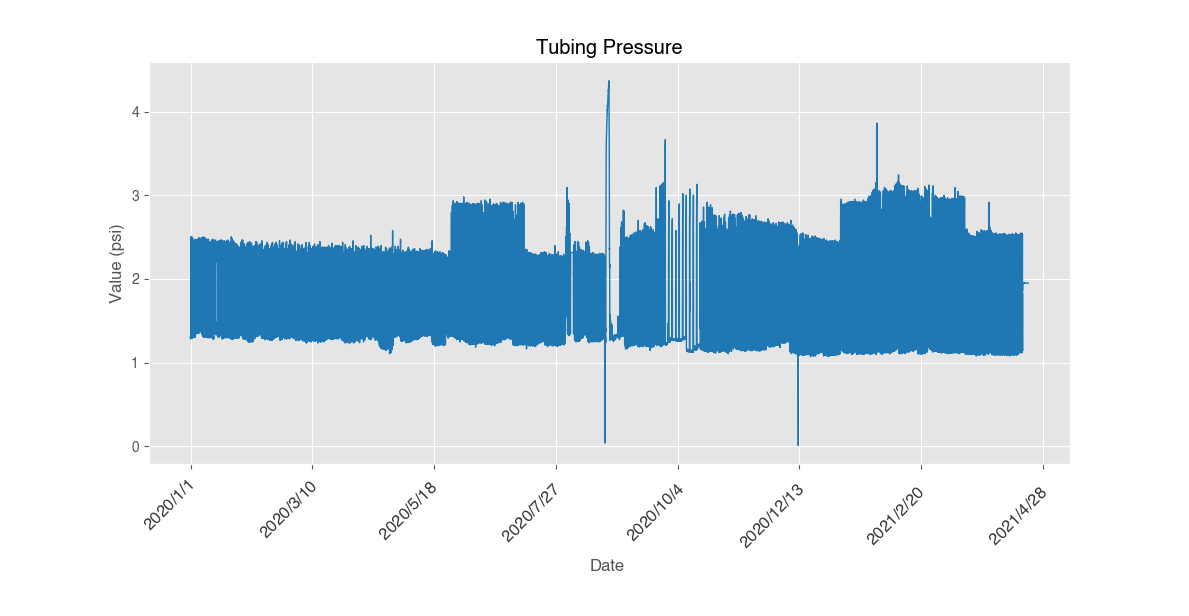
\includegraphics[width=12cm]{image/Figure_2.png}
    \caption{\centering Tubing pressure value changes during the process of plunger lift}
    \label{fig:tubing pressure}
\end{figure}

\subsection{Data Description}\label{subsec2}

Tubing pressure is the residual pressure left after the flow pressure lifts the oil and gas from the well bottom through the tubing to the wellhead, as measured by the tubing pressure gauge. The value of tubing pressure is determined by the flow pressure, friction resistance, and slippage loss of the oil-gas mixture column in the well. The pressure level of the oil is primarily dependent on the flow pressure, which is in turn related to the pressure of the oil layer. Therefore, the tubing pressure serves as a qualitative indicator of the well's energy. Casing pressure, on the other hand, is the pressure exerted by the surrounding ground on the well's casing. When controlled properly, casing pressure facilitates a consistent moving fluid level, thus improving the overall production rate of the well. Air pressure, in this context, refers to the pressure that a gas experiences as it passes through gas collection ground equipment and enters the gas pipeline. Flow rate denotes the quantity of fluid or gas that flows through a given section over a certain period, as measured by the rate of gas oil flow within the tubing. 

After a certain period of exploiting the gas well, the implementation of plunger lift became vital to prevent liquid loading and ensure continued production. Throughout the plunger lift process, tubing pressure, casing pressure, air pressure and flow rate all undergo significant change, with varying trends observed over time, as illustrated in Figure 2

\begin{figure}[htp]
    \centering
    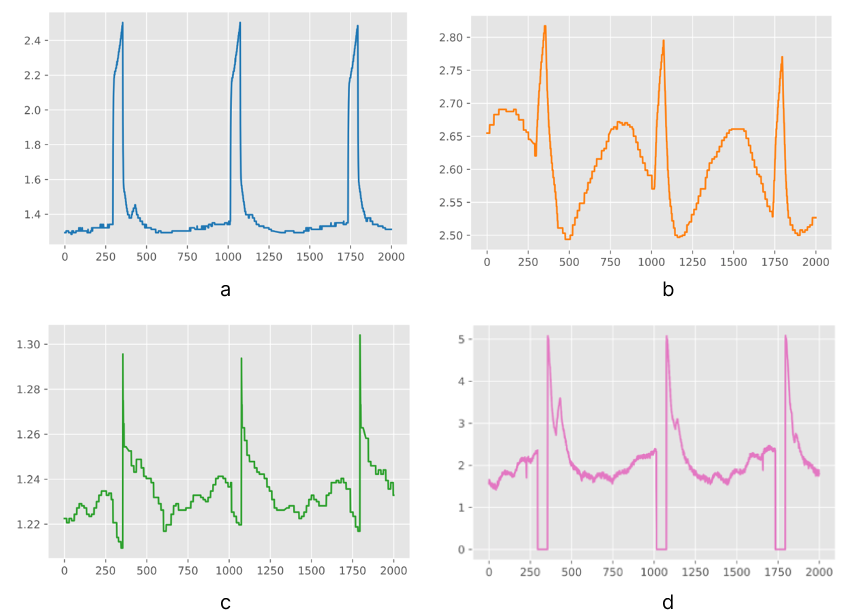
\includegraphics[width=12cm]{image/Frame 8.png}
    \caption{\centering Tubing pressure(a), casing pressure(b), air pressure(c) and flow rate(d) changes over time}
    \label{fig:four}
\end{figure}

Multivariate forecasting has been proven as an effective method to improve accuracy by increasing the value of information to a certain degree. In a study conducted by Niknam et al. (2023), forecasting water demand based on past consumption patterns using Multivariate-LSTM (MV-LSTM) coupled with average temperature showed higher accuracy and less error compared to Univariate-LSTM (UV-LSTM), which relied solely on lagged monthly average water consumption. Similarly, Wei et al. (2023) conducted comparative research on ultra-short-term wind power prediction and found that considering both historical series of wind power and wind speed resulted in a model with fewer errors than only considering historical series of wind power. When it comes to multi-dimensional input forecasting, taking into account the data correlation can increase the effective information of the data and avoid integrating redundant information that may negatively affect the forecast model and unnecessarily consume computing resources. Principal Component Analysis (PCA) is a statistical method that can calculate the correlation among data and present relative coefficients. By using the dimension-reduction concept, PCA transforms multiple variables into a few comprehensive variables. Each principal component can reflect the majority of the information contained in the original variables without repetition (Zhang et al., 2022).

The results of the correlation analysis are visualized in Figure 3, where a heatmap displays the coefficients of correlation between each pair of features. The degree of correlation is represented by a gradient of colors ranging from dark to light. A coefficient of 1 indicates a fully self-correlated relationship, while 0 denotes no correlation between the two features. If the correlation coefficient is close to either end of the spectrum, it means that one of the features is redundant and should be discarded to improve the accuracy of the forecasting model. In the case of forecasting tubing pressure, the correlation coefficients between tubing pressure and the other features are 1, 0.39, -0.22, and -0.48. None of these coefficients falls near either end of the correlation spectrum, which indicates that all four features are valuable inputs for the forecasting model.

\begin{figure}[htp]
    \centering
    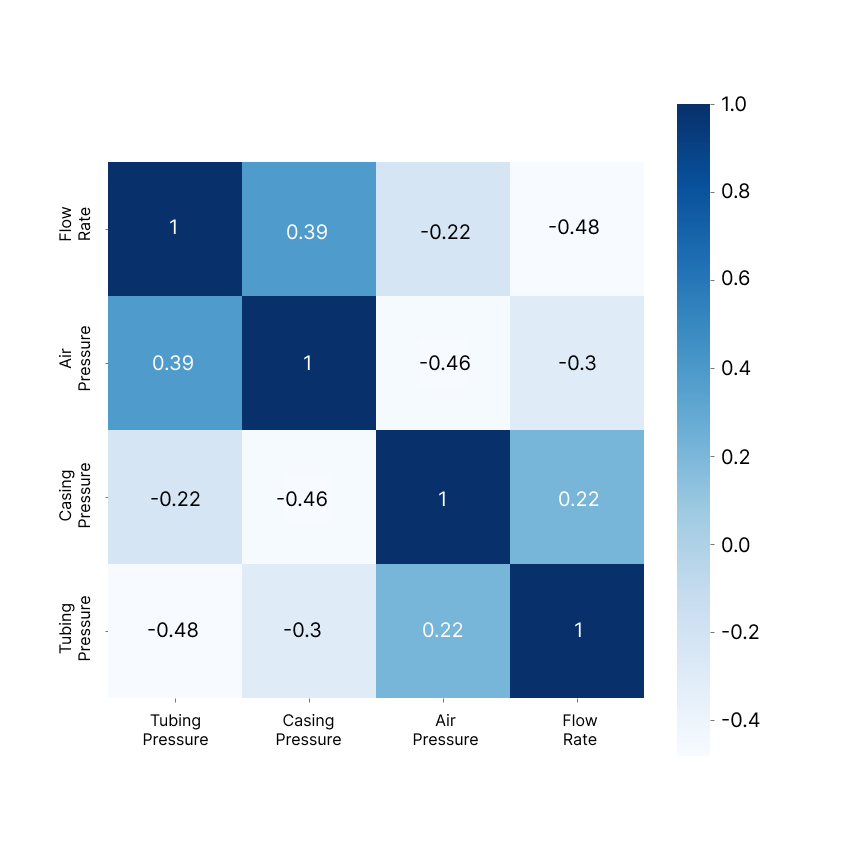
\includegraphics[width=10cm]{image/Frame 7.png}
    \caption{\centering Heatmap of PCA of Multi-dimensional input feature}
    \label{fig:PCA}
\end{figure}

Table 1 shows the exact start date and end date of each feature and respective data quantity.

\begin{table}[h]
\caption{An overview of experimental data}\label{tab1}%
\begin{tabular}{@{}llll@{}}
\toprule
Feature & Start Date  & End Date & Data Quantity\\
\midrule
Tubing Pressure    & 2020/1/1 00:00   & 2021/4/22 16:45  & 687,886  \\
Casing Pressure    & 2020/1/1 00:00   & 2021/4/22 16:46  & 687,887  \\
Air Pressure    & 2020/1/1 00:00   & 2021/4/22 16:46  & 687,887  \\
Flow Rate    & 2020/1/1 00:00   & 2021/4/22 16:43  & 687,884  \\
\botrule
\end{tabular}
\end{table}

\section{Proposed method}\label{sec3}

\subsection{Time Series Forecasting and statistical methods}\label{subsec3}

A time series is a statistical series that arranges the values of an indicator in chronological order. Conducting time series analysis enables us to gain insights into various data features such as long-term trends, seasonal changes, cyclical changes, and irregular changes. In many fields such as business (Kim, 2003), energy (Dudek, 2016), and environment (Araújo et al., 2017), predicting future trends is a vital task. Accurate time series forecasting can immensely benefit companies in terms of saving time and money by facilitating effective planning, scheduling, and other essential activities.

Traditional time series forecasting uses statistical methods. The well-established and accurate algorithm for analyzing and forecasting time series data is the Box-Jenkins method (Yip et al., 2014), and its commonly used models include: autoregressive model (AR model), sliding average model (MA model), (autoregressive-sliding average hybrid model) ARMA model, (differential integrated moving average autoregressive model) ARIMA model, where ARIMA model is a combination of former models. The ARIMA model is characterized by three important parameters, namely p, d, and q, which are discussed and presented below:

\begin{equation}
{({1 - {\sum\limits_{i = 1}^{p}\varnothing_{i}}L^{i}})}\left({1 - L} \right)^{d}X_{t} = \left({1 + {\sum\limits_{i = 1}^{q}{\theta_{i}L^{i}}}} \right)\varepsilon_{t}
\end{equation}

Where p represents the autoregressive term, d represents the number of differences made when the time series became stationary, q represents the number of moving average items and L is the lag operator.

Yamacli et al. (2023) conducted a comparative study on estimating the unemployment rate in Turkey. They compared two models - ARIMA and machine learning - including Covid-19 pandemic periods. The results revealed that ARIMA was more appropriate for estimating the unemployment rate before the pandemic, since the data was relatively linear-based during that time. However, during the intense pandemic period from 2020-2021, where the data was highly affected by economic uncertainty from various aspects of society, ARIMA showed a higher forecasting error than the machine learning model. This is likely due to the non-linear characteristic of the data. Teams from Turkey conducted a compelling case study on predicting electricity demand – a vital aspect in determining the number of storage devices and their capacity for grid systems. The study compared two forecasting methods: Auto Regressive Integrated Moving Average (ARIMA) and Artificial Neural Network (ANN) for predicting electricity load. The results showed that both methods can estimate consumption, but ANN proved to be more proficient in handling non-linear data structures as opposed to ARIMA, which was limited to linear data structures (Chafak et al., 2023).

Although the ARIMA model boasts simplicity by requiring only endogenous variables and no need for exogenous variables, it has limitations when dealing with data. There are two main limitations: First, the time series data must be stationary or stable through differencing. Second, the model can only capture linear relationships and is unable to handle non-linear relationships. In the case of processing production data for the plunger lift process, which exhibits a noticeable trend and periodicity, the ARIMA model is insufficient to address relevant issues.

\subsection{Recurrent neural networks}\label{subsec4}

With the constant advancements in chip technology and related fields, the performance of central processing units (CPUs) and graphic processing units (GPUs) has improved dramatically. This has effectively eliminated any previous restrictions on computing resources and has allowed researchers to shift their focus towards the development of artificial neural networks to tackle real-world problems. However, conventional artificial neural networks, such as Recurrent Neural Networks (RNNs), face significant challenges when it comes to extracting meaningful information from historical data and adapting to changes in features across various time scales. On the other hand, the Long Short-Term Memory (LSTM) network can effectively overcome these limitations and provide an efficient solution for these issues.

\begin{figure}[htp]
    \centering
    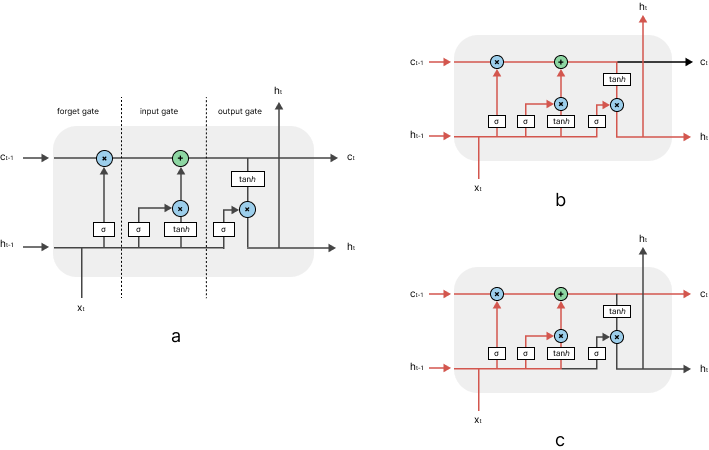
\includegraphics[width=10cm]{image/Frame 3.png}
    \caption{\centering  Structure and information flow within Long Short-Term Memory cell}
    \label{fig:LSTM}
\end{figure}

 Long Short-Term Memory (LSTM) is a critical component of Recurrent Neural Networks (RNNs), first introduced by Sepp Hochreiter and Jürgen Schmidhuber (1996). Researchers have utilized LSTM to solve various issues across many fields, and the progress of developing and enhancing LSTM is still ongoing. Compared to RNNs, LSTM offers numerous advantages, particularly in overcoming the vanishing gradient problem commonly encountered in classic RNN networks (Yanuar, 2018). Moreover, the unique capability of LSTM in retaining information and detecting patterns from past time periods makes it an ideal choice for long-term dependent learning tasks. This remarkable ability is attributed to its advanced hidden structure, as shown in Figure 4A, which includes a long-term state ct and three selective gates: forget gate, input gate, and output gate, operating at a given time step. This mechanism sets it apart from conventional RNNs. Simple RNNs, such as the Elman network, rely solely on the hidden state ht as the short-term state. However, in an LSTM layer, both the short-term state ht and long-term state ct are utilized, enabling the learning of short- and long-term patterns in longer sequences. Furthermore, the forget gate is responsible for discarding memories, while the input gate introduces new ones, and the output gate filters the outcomes as the long-term state traverses through the network. Figure 4B and C demonstrate how the current moment state ht and ct are influenced and shaped through the cell.

 Led by Zha et al. (2022), the research team aimed to predict gas field production, and experimented with various forecasting models including CNN (Convolutional Neural Network), RNN, and ARIMA. Among these models, the CNN-LSTM combination emerged as the most effective, indicating LSTM's ability to extract information from a previous sequence. Nevertheless, the team also found out that a model consisting solely of LSTM had lower performance. This finding underscores the fact that while LSTM possesses a robust capacity to learn from the past, it cannot achieve optimal results on its own. Its performance is optimized when combined with other units.

\subsection{Autoenocoder}\label{subsec5}


Autoencoder is an effective unsupervised method for compressing data dimensions and expressing data features. It comprises a non-recurrent feed-forward neural network composed of an input layer, an output layer, and a set of hidden layers (Gopikrishnan et al., 2023). The input and output layers consist of the same number of neurons. Autoencoders are trained using two functions - encoder and decoder - to reconstruct input data at the output nodes. The encoder function maps a lengthy vector to a lower-dimension vector and repeats this process for multiple layers, compressing the data dimensions and extracting abstract features. Figure 5 depicts the content density of data information and how it increases during this process, represented by the color change from yellow to red. The decoder function, on the other hand, reconstructs the input data fed by the encoder back into its original shape and dimension. Together, they transform the vector into a more organized and information-oriented form. Figure 5 demonstrates how the block filled with diagonal lines represents the desired information, albeit located in a disordered and scattered fashion. However, autoencoder encoding and decoding make the information block more concentrated and organized, facilitating further feature extraction of other structures within the recurrent neural network. 

\begin{figure}[htp]
    \centering
    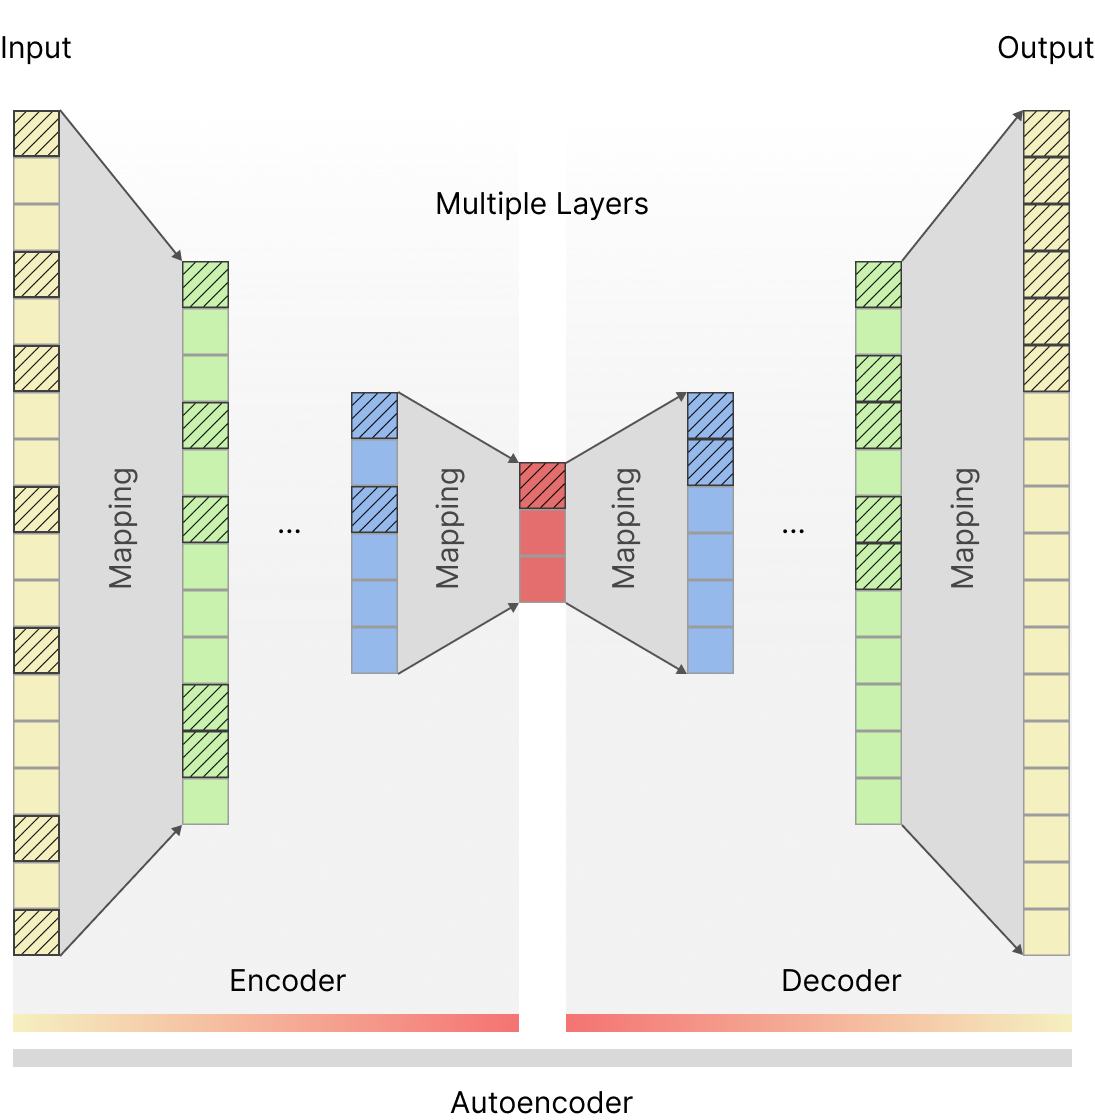
\includegraphics[width=8cm]{image/Frame 6.png}
    \caption{\centering  Structure of autoencoder}
    \label{fig:autoencoder}
\end{figure}

Li et al. (2023) conducted a thorough analysis of different types of autoencoders and their variations, all of which have shown great potential in image classification, object detection, and natural language processing[29]. The autoencoder's ability to efficiently extract and compress information across one or multiple dimensions has been extensively validated. Zhou et al. (2022) introduced a novel contrastive autoencoder that was utilized for anomaly detection in multivariate time series data. The experimental findings suggest that this new approach significantly outperforms the baseline models. Furthermore, the visualization of learned representations demonstrates its capacity to model normal data patterns.

\subsection{Problem Statement}\label{subsec6}


The data is sampled every minute, which means that to enable early warning, planning, and other purposes, the forecasting data needs to span a sufficient length. This will give gas well personnel enough time to accurately assess and respond to potential issues. Our goal is to calculate the values of the forecasting time span, which forms a set
\begin{equation}
P=[ k1, k2, …, kn]
\end{equation}
where n is the number of minutes ahead of the current moment, k0. However, it is crucial to strike a balance as an excessively large n will negatively impact the accuracy of predictions, rendering them ineffective on production monitoring. Conversely, an overly small n can ensure model predictions' accuracy, but it will limit the time available for workers to assess and respond to potential issues, rendering the entire forecast ineffective. Thus, finding an optimal n is essential for effective forecasting.


To achieve the target for set P, the historical data that is fed into the model must be carefully considered. set 
\begin{equation}
H=[ k-m, k-m+1, …, k-1 ]
\end{equation}
with the value for m requiring confirmation. Ideally, all available historical data would be used to enhance the accuracy of the model. However, practical considerations such as computing resources and time constraints may require a compromise between model precision and efficiency. It is important to select an appropriate value for m that allows for the most accurate model predictions while ensuring timely execution.

The single-step forecasting strategy, commonly used in oil and gas production forecasting, demonstrates high accuracy in monthly shale gas production forecasting at Duvernay Formation (Lee et al., 2019). Its extension, the recursive multi-step forecasting strategy, utilizes past prediction data as known history to forecast the next month and repeats this process to achieve the desired time span. While this approach guarantees the intended forecasting length, it heavily relies on the correct historical data, leading to potentially significant deviation if even a small error exists in the earlier part of set T. Figure 6 demonstrates that the accuracy of the recursive multi-step forecasting strategy decreases as the forecasting horizon increases, resulting from the accumulated prediction errors.

\begin{figure}[htp]
    \centering
    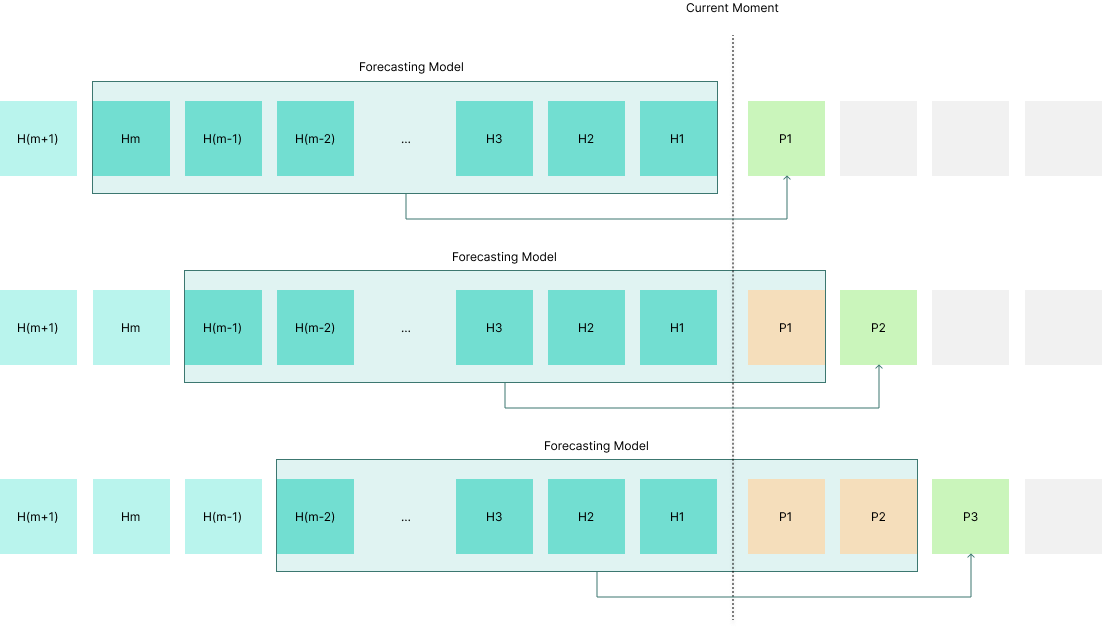
\includegraphics[width=8cm]{image/Frame 9.png}
    \caption{\centering  Recursive Multi-step Forecasting Strategy}
    \label{fig:recursive}
\end{figure}

Given the stringent demand for precise historical data in the recursion-based multi-step forecasting strategy, it is not feasible for the forecasting model to sustain optimal accuracy throughout the entire forecasting range. To contend with this limitation, a multiple-output forecasting scheme is adopted wherein the forecasting model directly predicts the future set P based on the provided historical dataset H, as illustrated in Figure 7.

\begin{figure}[htp]
    \centering
    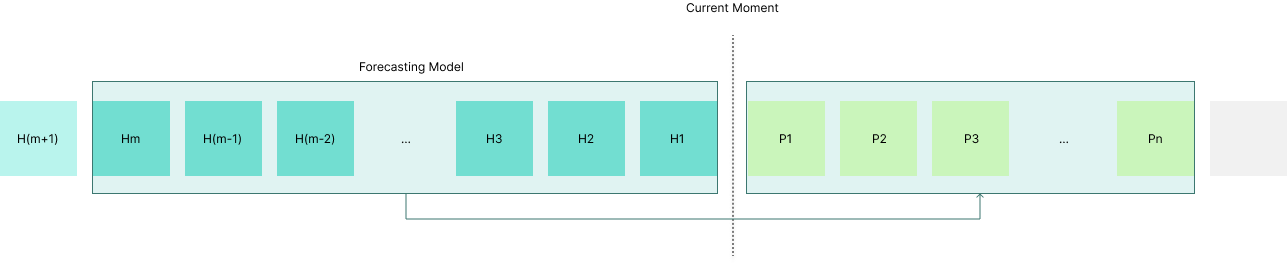
\includegraphics[width=8cm]{image/Frame 10.png}
    \caption{\centering  Multiple Output Forecasting Strategy}
    \label{fig:multiple output}
\end{figure}

\subsection{Method Overview}\label{subsec7}

\begin{figure}[htp]
    \centering
    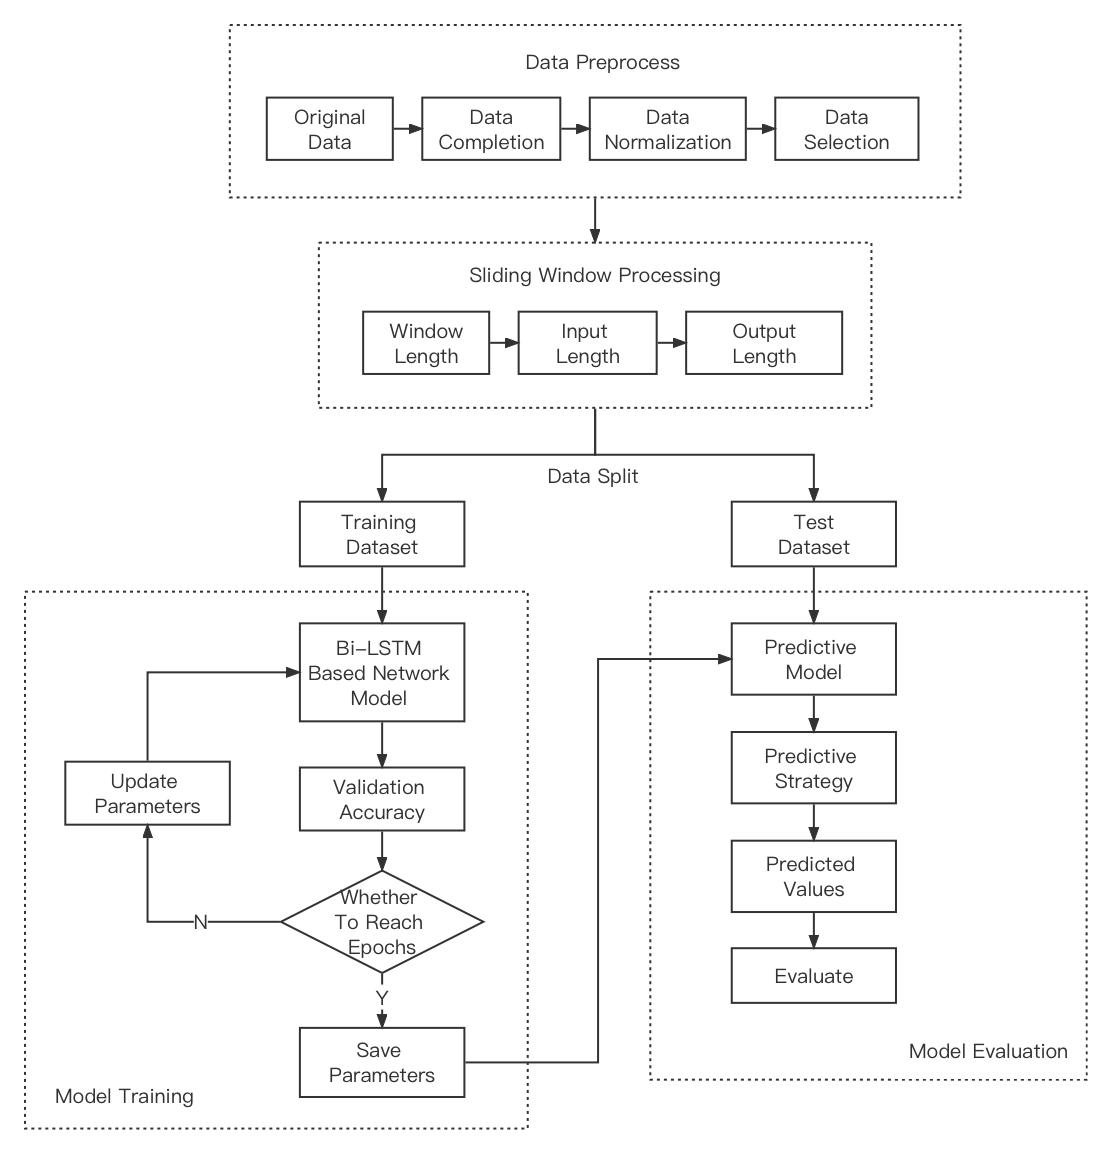
\includegraphics[width=10cm]{image/flowchart.png}
    \caption{\centering  Workflow of overall methods}
    \label{fig:workflow}
\end{figure}

As seen in Figure 8, the whole workflow mainly consists of 5 parts: data preprocessing, sliding window processing, data split, model training and model evaluation.


Due to the complex and unstable nature of on-site working conditions, there may be instances of individual abnormal situations occurring on the monitoring equipment, resulting in some time nodes of the feature not being recorded. This creates a hiatus in the time series, making data completion necessary during the preprocessing phase in order to fill in the blanks and ensure the continuity of the time series. Additionally, the dataset features have varying value ranges, which can cause the gradient to fluctuate during model training, resulting in a longer time to reach the local or global optimal value. To address this issue, data normalization is used to ensure that all features are on the same metric scale. In this study, the research focuses on the features of normal operating conditions of plunger lift, and therefore, abnormal conditions such as liquid loading, stuck motor valve, exploitation suspension, etc. should not be considered. Data selection is used to eliminate these abnormal parts and choose the relatively non-volatile parts from January 1st, 2020 to April 10th, 2020, totaling to a hundred days. Moreover, the abnormal conditions display distinct numerical changes that deviate from the normal conditions, such as an out-of-range and continuous increase, as depicted in Figure 9.

\begin{figure}[htp]
    \centering
    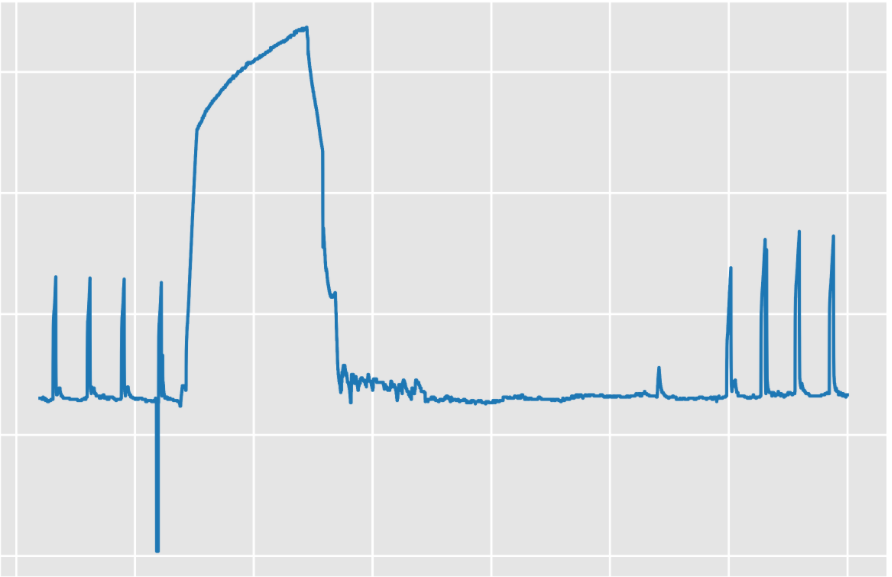
\includegraphics[width=8cm]{image/error.png}
    \caption{\centering  A typical abnormal operating conditions}
    \label{fig:abnormal}
\end{figure}

The time series data will be segmented and arranged into a format suitable for neural networks by means of sliding window processing, based on our specific requirements, as shown in figure 10. Two important parameters that can significantly impact the training efficiency and predictive accuracy of the model are the length of historical data (m) and forecasting data (n). After conducting experiments, we have found that the appropriate length for historical data is 800, which is sufficient to cover one period of an individual feature, thus enabling the model to capture the characteristic trends of the data. However, it should not be too long to hinder the learning process. For forecasting data, the appropriate length is 200, approximately 3 hours ahead of time. This allows ample time for working staff to make judgement calls and prepare reactions accordingly.

\begin{figure}[htp]
    \centering
    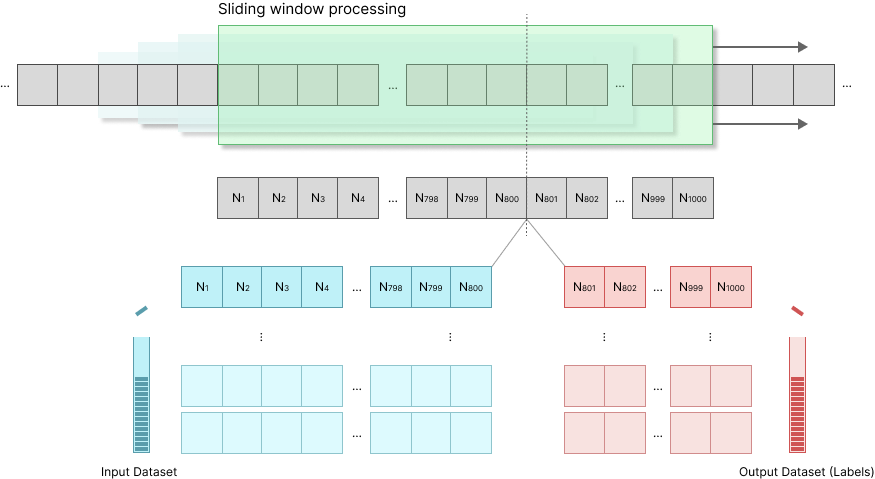
\includegraphics[width=10cm]{image/Frame 11.png}
    \caption{\centering  Sliding window processing}
    \label{fig:window}
\end{figure}


After the sliding window processing, the time series with a selected length of 144,000 was divided into a history data set H (800,1) and a corresponding prediction data set P (200,1) that were combined into a group. A total of 143,000 groups were then divided into training, validation, and test data sets with a ratio of 0.8:0.1:0.1, resulting in 114,400 groups for training data, 14,300 groups for validation data, and 14,300 groups for test data to be used in the later stages of evaluation. 


During model training, neural network parameters were adjusted according to validation accuracy via gradient descent iterations to approach optimal values. The best combination of neural network parameters and model were automatically saved for later evaluation. 

\begin{figure}[htp]
    \centering
    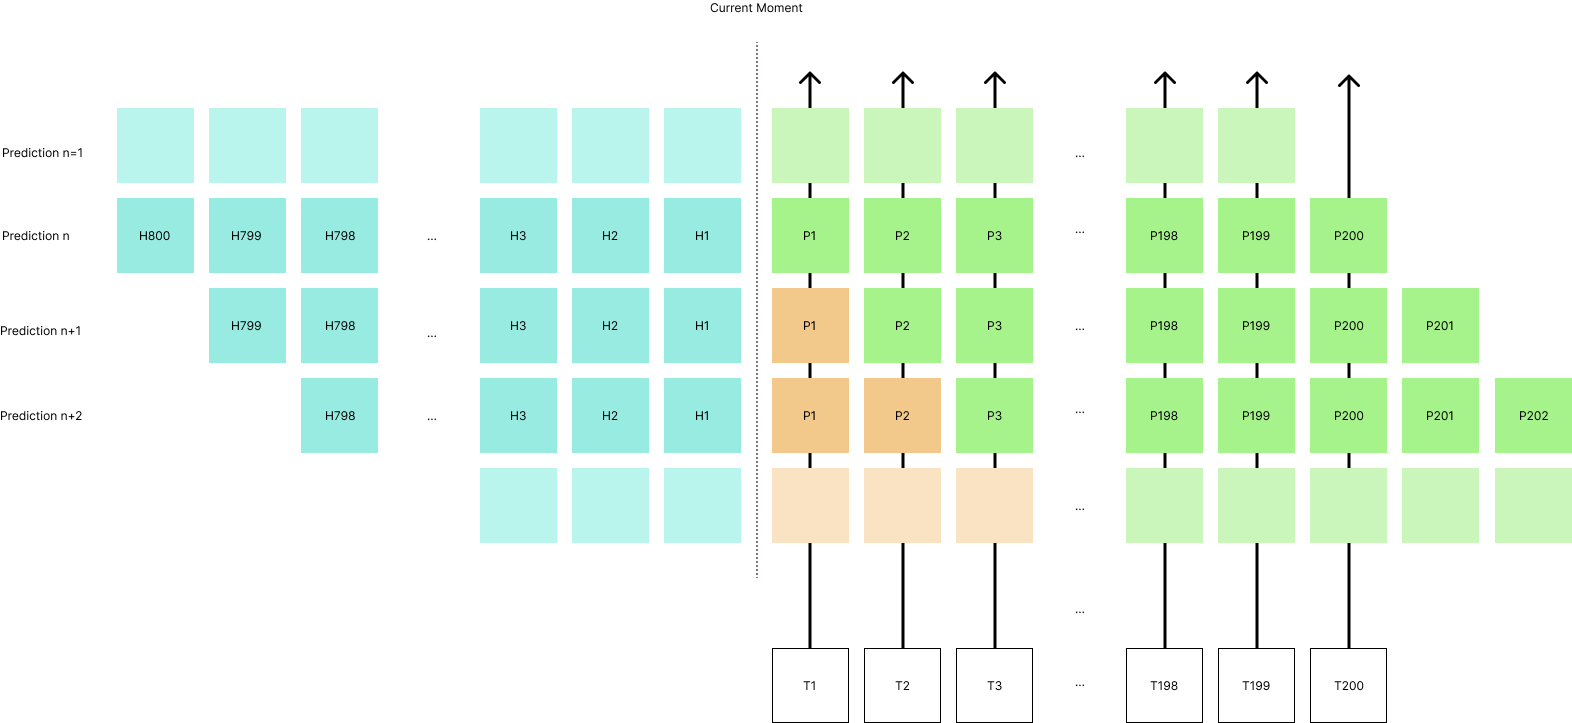
\includegraphics[width=10cm]{image/Frame 1.png}
    \caption{\centering  Rolling forecasting strategy}
    \label{fig:rolling}
\end{figure}

To counteract possible fluctuations and abnormalities in forecasting data, an innovative predictive strategy called rolling forecasting was employed. This involved combining multiple predictions of the same time tick and assigning relative weights to individual values to calculate the representative value for that time tick, as depicted in Figure 11.


Define the present moment as T0, {T1, T2, T3, …, T200} is the set of time node of which respective values we are attempting to acquire. For prediction n, light green values {P1, P2, P3, …, P200} are the forecasting data we get from predictive model by inputting light blue values {H1, H2, H3, …, H800}, which are the history data. For the next prediction, n+1, we take the forecasting data of P1 and include it temporarily as a known data point within the predictive model. This enables us to obtain the next set of forecasting data, {P2, P3, P4, …, P201}, which can be used for further predictions, and so on. Depending on the position of each time node in relation to the current moment, up to 200 predictions can be generated, each with a relative weight assigned to it. These weights are then used to calculate a representative value for each time node.

\subsection{Evaluation Criteria}\label{subsec8}

Evaluation indicators of the forecasting model contain two perspectives, the error and the accuracy of the model prediction results. For the former one, root mean square error (RMSE) (Zhu et al., 2020), average absolute error (MAE) (Yuan et al., 2017) and mean absolute percentage error (MAPE) (Putz et al., 2021) are considered. For the latter one, R2 score and predictive graph compared with actual one are both considered. The specific definition are as follows:

\begin{equation}
RMSE = \frac{1}{C_{Ni}}\sqrt{\frac{1}{n}{\sum\limits_{k = 1}^{n}\left( y_{ki} - {\hat{y}}_{ki} \right)^{2}}}
\end{equation}

\begin{equation}
MAE = \frac{1}{nC_{Ni}}{\sum\limits_{k = 1}^{n}\left| {y_{ki} - {\hat{y}}_{ki}} \right|}
\end{equation}

\begin{equation}
sMAPE = \frac{100\%}{n}{\sum\limits_{k = 1}^{n}\frac{\left| {y_{ki} - {\hat{y}}_{ki}} \right|}{\left| {y_{ki} + {\hat{y}}_{ki}} \right|/2}}
\end{equation}

\begin{equation}
R^{2} = 1 - \frac{\sum\limits_{k = 1}^{n}\left( {y_{ki} - {y\hat{y}}_{ki}} \right)^{2}}{\sum\limits_{k = 1}^{n}\left( {y_{ki} - {\overset{-}{y}}_{i}} \right)^{2}}
\end{equation}

where $y_{ki}$ and ${\hat{y}}_{ki}$ represent the actual value and predicted value of tubing pressure at time k in predicted scenario i, respectively. $y_{i}$ represents the average value of the actual value in predicted scenario i, n represents the total number of data within this interval.

\section{Results and Discussion}\label{sec4}

\begin{figure}[htp]
    \centering
    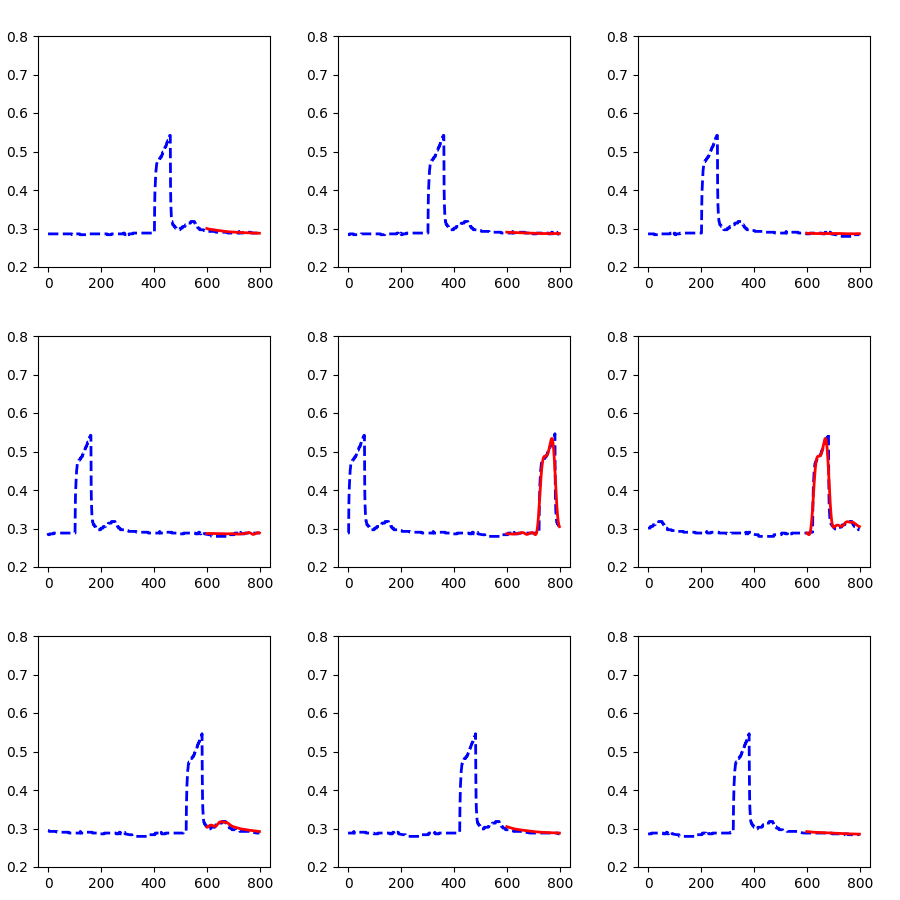
\includegraphics[width=8cm]{image/Frame 2.png}
    \caption{\centering Forecasting results starting with different time nodes}
    \label{fig:9}
\end{figure}

\begin{figure}[htp]
    \centering
    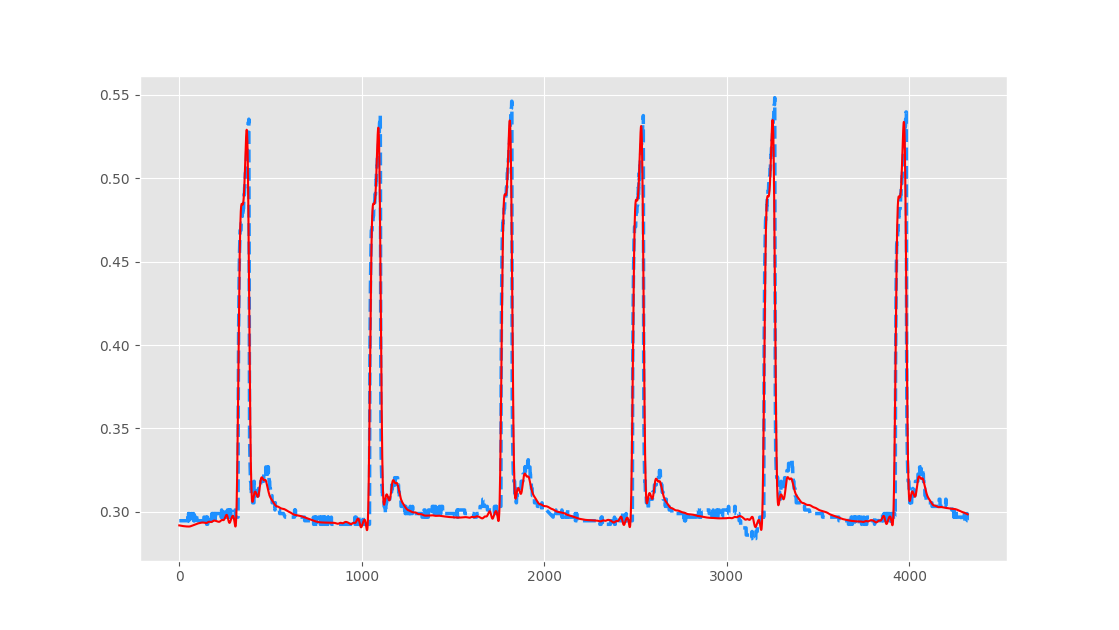
\includegraphics[width=10cm]{image/plot.png}
    \caption{\centering  Consistent forecasting presentation}
    \label{fig:consistent}
\end{figure}

The forecasting data presented in Figure 12 demonstrates the robustness of the predictive model to the periodicity of the objective feature, tubing pressure. The results show that different starting time nodes along the feature have been considered and the model is able to accurately predict the location and range of both the peak and subsequent small wave peak at the bottom of the tubing pressure chart. This consistency in accuracy across different starting time nodes is particularly important as it indicates that the predictive model is able to account for variations in the initial conditions of the system. Along the timeline, the overall forecasting result was presented in figure 13, which was a small segment extracted from the test set. The effective minimization of errors in the predictive model is also worth noting, as it suggests that the model is able to effectively capture the underlying dynamics of the system. This accuracy in forecasting can have significant implications for the efficiency and productivity of plunger lift systems, as it can enable operators to make informed decisions and optimize the performance of their systems.

\begin{figure}[htp]
    \centering
    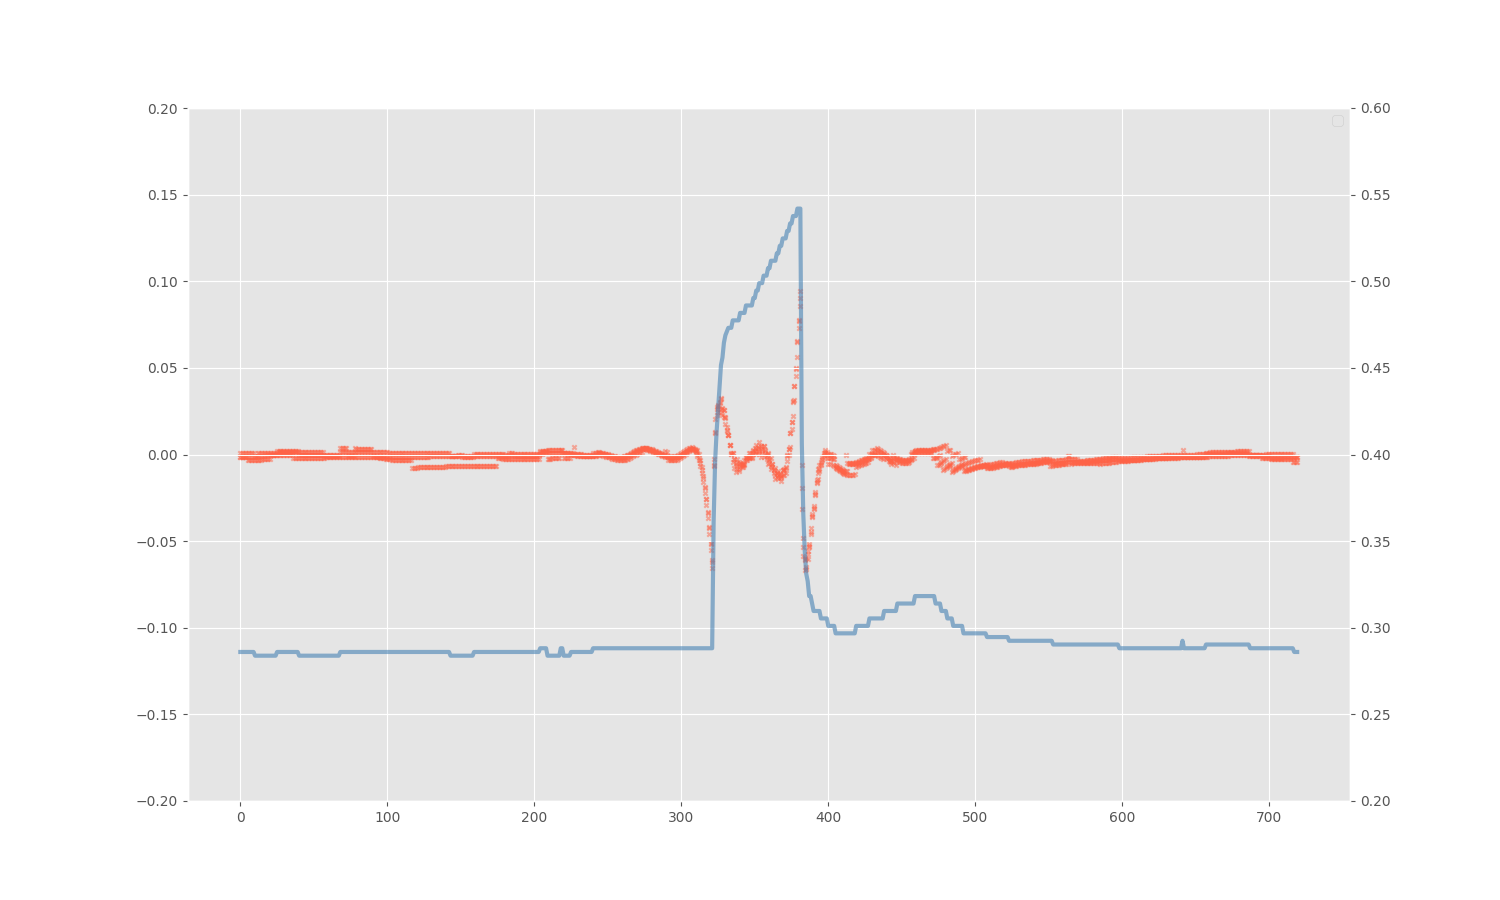
\includegraphics[width=10cm]{image/error_distribution.png}
    \caption{\centering  Distribution of the error along the cycle}
    \label{fig:distribution}
\end{figure}

Figure 14 displays the distribution of error deviation between model forecasting data and the actual value during the plunger lift cycle. It is evident that the most significant deviation occurs at the peak of the tubing pressure. Upon closer examination of the forecasting figure, it can be deduced that the deviation is due to the model's advance factor. The forecasting model predicts the peak slightly before the actual moment, leading to this deviation. However, the error is minimal and stable for other sections of the cycle.

\begin{table}[h]
\caption{Evaluation indicators of error and accuracy}\label{tab2}%
\begin{tabular}{l l l l l l}
\toprule
Model & RMSE  & MAE & MAPE & $R^{2}$ & \\
\midrule
ABILSTM    & 1.09   & 0.47  & 1.40 & 96.97 & \\
BILSTM-AE     & 1.20   & 0.49  & 1.46 & 95.49 & \\
SBILSTM    & 0.95   & 0.50  & 1.12 & 96.38 & \\
CBILSTM     & 1.73   & 0.68  & 1.96 & 90.68 &\\
BILSTM     & 1.21   & 0.62  & 1.90 & 95.30 & \\
LSTM       & 1.47   & 0.69  & 2.45 & 93.09 & \\
GRU       & 1.31   & 0.72  & 2.23 & 94.46 & \% \\

\botrule
\end{tabular}
\end{table}

The results from Table 2 clearly demonstrate the superior performance of the noise smooth bidirectional LSTM (SBILSTM) architecture, which achieved the lowest error rate of 0.95\% and an impressive R2 score of 96.38\%. The multi-forecast average bidirectional LSTM (ABILSTM) model also showed remarkable performance, with an error rate of only 1.09\% and an R2 score of 96.97\%, which was the highest among all the models considered. In particular, the rolling forecasting strategy applied to ABILSTM resulted in a significant reduction of approximately 10\% in error rate and an improvement of 1.75\% in R2 score, compared with the traditional bidirectional LSTM (BILSTM) model. When considering both statistical data and visual agreement with the graph, ABILSTM demonstrated superior performance over all the other models, indicating its potential for practical applications in financial forecasting and analysis. These results suggest that both SBILSTM and ABILSTM can be effective approaches for modeling financial data, and that incorporating rolling forecasting strategies can further improve their performance.

\section{Conclusion}\label{sec5}

In this study, a novel approach for predicting tubing pressure during the process of plunger lift was proposed, based on a bidirectional long-short term memory (Bi-LSTM) model. The model was able to learn the inherent characteristics and trends of tubing pressure changes over time, by utilizing recurrent neural networks formed with bidirectional LSTM cells. To enhance the accuracy and efficiency of the predictions, a multi-dimensional approach was adopted, incorporating a rolling forecasting strategy that effectively utilized the available data and eliminated fluctuations in the forecasting results. The experimental results and evaluations demonstrated that the proposed model achieved comparable performance with contemporary methods for time series prediction. To further highlight the potential of the approach, future studies will focus on combining time series forecasting of tubing pressure with anomaly detection and classification. This approach will enable the examination and analysis of anomalous conditions, which can then be used to improve the structure of the neural networks, leading to more accurate predictions. By incorporating anomaly detection into the forecasting process, the workload of working staff can be greatly reduced, and monitoring costs can be minimized. Overall, the proposed approach presents a promising solution for predicting tubing pressure during the plunger lift process, which could have significant applications in the oil and gas industry.




%%=============================================%%
%% For presentation purpose, we have included  %%
%% \bigskip command. please ignore this.       %%
%%=============================================%%




%%=============================================%%
%% For presentation purpose, we have included  %%
%% \bigskip command. please ignore this.       %%
%%=============================================%%

%%=============================================%%
%% For presentation purpose, we have included  %%
%% \bigskip command. please ignore this.       %%
%%=============================================%%


%%=============================================%%
%% For presentation purpose, we have included  %%
%% \bigskip command. please ignore this.       %%
%%=============================================%%

%%=============================================%%
%% For presentation purpose, we have included  %%
%% \bigskip command. please ignore this.       %%
%%=============================================%%


%%=============================================%%
%% For presentation purpose, we have included  %%
%% \bigskip command. please ignore this.       %%
%%=============================================%%

%%=============================================%%
%% For presentation purpose, we have included  %%
%% \bigskip command. please ignore this.       %%
%%=============================================%%

%%=============================================%%
%% For presentation purpose, we have included  %%
%% \bigskip command. please ignore this.       %%
%%=============================================%%


%%===================================================%%
%% For presentation purpose, we have included        %%
%% \bigskip command. please ignore this.             %%
%%===================================================%%


%%\begin{appendices}

%%\section{Section title of first appendix}\label{secA1}

%%An appendix contains supplementary information that is not an essential part of the text itself but which may be helpful in providing a more comprehensive understanding of the research problem or it is information that is too cumbersome to be included in the body of the paper.

%%=============================================%%
%% For submissions to Nature Portfolio Journals %%
%% please use the heading ``Extended Data''.   %%
%%=============================================%%

%%=============================================================%%
%% Sample for another appendix section			       %%
%%=============================================================%%

%% \section{Example of another appendix section}\label{secA2}%
%% Appendices may be used for helpful, supporting or essential material that would otherwise 
%% clutter, break up or be distracting to the text. Appendices can consist of sections, figures, 
%% tables and equations etc.

%%\end{appendices}

%%===========================================================================================%%
%% If you are submitting to one of the Nature Portfolio journals, using the eJP submission   %%
%% system, please include the references within the manuscript file itself. You may do this  %%
%% by copying the reference list from your .bbl file, paste it into the main manuscript .tex %%
%% file, and delete the associated \verb+\bibliography+ commands.                            %%
%%===========================================================================================%%

\bibliography{sn-bibliography}% common bib file
%% if required, the content of .bbl file can be included here once bbl is generated
%%\input sn-article.bbl

A. r. Yanuar, “Recurrent Neural Network(RNN),” 1 Juli 2018. [Online]. Available: https://machinelearning.mipa.ugm.ac.id/2018/07/01/recurrent-neural-network-rnn/.

Adesina Fadairo,Falode Olugbenga \& Nwosu Chioma Sylvia.(2015).A new model for predicting liquid loading in a gas well. Journal of Natural Gas Science and Engineering(C). doi:10.1016/j.jngse.2014.09.003.

Chava, G. K., Falcone, G., \& Teodoriu, C. (2008, September). Development of a New Plunger-Lift Model Using Smart Plunger () Data. In SPE Annual Technical Conference and Exhibition. OnePetro.

Chen Yan,Huang Yunan,Miao Bo,Shi Xiangchao \& Li Ping.(2022).Adaptive anomaly detection-based liquid loading prediction in shale gas wells. Journal of Petroleum Science and Engineering. doi:10.1016/J.PETROL.2022.110522. 

G. Dudek, Neural networks for pattern-based short-term load forecasting: A comparative study, Neurocomputing 205 (2016) 64–74, https://doi.org/ 10.1016/j.neucom.2016.04.021.

Gasbarri Sandro \& Wiggins Michael L..(2001).A Dynamic Plunger Lift Model for Gas Wells. SPE Production \& Facilities(02). doi:10.2118/72057-PA.

Gopikrishnan, C. P., \& Madhavan, M. (2023). Denoising Autoencoder based Long non-coding RNA-Disease Association Prediction. Procedia Computer Science, 218, 836-844.

Han-Young Park,Gioia Falcone \& Catalin Teodoriu.(2009).Decision matrix for liquid loading in gas wells for cost/benefit analyses of lifting options. Journal of Natural Gas Science and Engineering(3). doi:10.1016/j.jngse.2009.03.009.

He Zhang,Gioia Falcone \& Catalin Teodoriu.(2010).Modeling fully transient two-phase flow in the near-wellbore region during liquid loading in gas wells. Journal of Natural Gas Science and Engineering(2). doi:10.1016/j.jngse.2010.04.005.

Hernandez, A., Maracano, L., Caicedo, S., \& Cabunaru, R. (1993, October). Liquid fall-back measurements in intermittent gas lift with plunger. In SPE Annual Technical Conference and Exhibition. OnePetro.

Hochreiter, S. , \& Jürgen Schmidhuber. (1996). Bridging long time lags by weight guessing and "long short term memory". spatiotemporal models in biological \& artificial systems.

Hon-lun Yip,Hongqin Fan \& Yat-hung Chiang.(2014).Predicting the maintenance cost of construction equipment: Comparison between general regression neural network and Box–Jenkins time series models. Automation in Construction. doi:10.1016/j.autcon.2013.10.024.

K. Kim, Financial time series forecasting using support vector machines, Neurocomputing 55 (1) (2003) 307–319, https://doi.org/10.1016/S0925-2312 (03)00372-2.

Lea, J. F., \& Rowlan, L. (2019). Gas well deliquification. Gulf Professional Publishing. 

Lee, K. ,  Lim, J. ,  Yoon, D. , \&  Jung, H. . (2019). Prediction of shale-gas production at duvernay formation using deep-learning algorithm. SPE Journal, 24(6).

Li, P., Pei, Y., \& Li, J. (2023). A comprehensive survey on design and application of autoencoder in deep learning. Applied Soft Computing, 110176.

Niknam Azar,Zare Hasan Khademi,Hosseininasab Hassan \& Mostafaeipour Ali.(2023).Developing an LSTM model to forecast the monthly water consumption according to the effects of the climatic factors in Yazd, Iran. Journal of Engineering Research(1). doi:10.1016/J.JER.2023.100028. 

Paulo J. Waltrich,Catalina Posada,Jessica Martinez... \& Jader R. Barbosa.(2015).Experimental investigation on the prediction of liquid loading initiation in gas wells using a long vertical tube. Journal of Natural Gas Science and Engineering(C). doi:10.1016/j.jngse.2015.06.023.

Putz, D., Gumhalter, M., Auer, H., 2021. A novel approach to multi-horizon wind power forecasting based on deep neural architecture. Renew. Energy 178, 494–505.

R. Araújo, A. Oliveira, S. Meira, On the problem of forecasting air pollutant concentration with morphological models, Neurocomputing 265 (2017) 91– 104, https://doi.org/10.1016/j.neucom.2017.01.107.

Sami Nagham Amer.(2022).Application of machine learning algorithms to predict tubing pressure in intermittent gas lift wells. Petroleum Research(2). doi:10.1016/J.PTLRS.2021.09.006.

Sayman O.,Jones K.,Hale R.,Pereyra E. \& Sarica C..(2021).A field case study of plunger lift related tubing deformation. Journal of Natural Gas Science and Engineering(prepublish). doi:10.1016/J.JNGSE.2021.104342.

Tang, Y. (2009, October). Plunger lift dynamic characteristics in single well and network system for tight gas well deliquification. In SPE Annual Technical Conference and Exhibition. OnePetro.

Tarmanini Chafak,Sarma Nur,Gezegin Cenk \& Ozgonenel Okan.(2023).Short term load forecasting based on ARIMA and ANN approaches. Energy Reports(S3). doi:10.1016/J.EGYR.2023.01.060.

Wei Junqiang,Wu Xuejie,Yang Tianming \& Jiao Runhai.(2023).Ultra-short-term forecasting of wind power based on multi-task learning and LSTM. International Journal of Electrical Power and Energy Systems. doi:10.1016/J.IJEPES.2023.109073.

Yamacli, D. S., \& Yamacli, S. (2023). Estimation of the unemployment rate in Turkey: A comparison of the ARIMA and machine learning models including Covid-19 pandemic periods. Heliyon, e12796.

Yuan, X., Tan, Q., Lei, X., Yuan, Y., Wu, X., 2017. Wind power prediction using hybrid autoregressive fractionally integrated moving average and least square support vector machine. Energy 129, 122–137.

Zha Wenshu,Liu Yuping,Wan Yujin,Luo Ruilan,Li Daolun,Yang Shan \& Xu Yanmei.(2022).Forecasting monthly gas field production based on the CNN-LSTM model. Energy. doi:10.1016/J.ENERGY.2022.124889.

Zhang, Z. ,  Sun, B. ,  Wang, Z. ,  Gao, Y. ,  Liu, S. , \&  Yin, Z. . (2018). Whole wellbore liquid loading recognition model for gas wells. Journal of Natural Gas Science \& Engineering.

Zhang Kuan,Chen Zehua,Yang Liyuan,Liang Yongchun. Principal component analysis (PCA) based sparrow search algorithm (SSA) for optimal learning vector quantized (LVQ) neural network for mechanical fault diagnosis of high voltage circuit breakers[J]. Energy Reports,2023,9(S1).

Zheng Tong,Xiaohan Pei,Zejun Shen... \& Haifeng Niu.(2015).A plunger lift and monitoring system for gas wells based on deployment-retrievement integration. Natural Gas Industry B(5). doi:10.1016/j.ngib.2015.09.021.

Zhou Hao,Yu Ke,Zhang Xuan,Wu Guanlin \& Yazidi Anis.(2022).Contrastive autoencoder for anomaly detection in multivariate time series. Information Sciences. doi:10.1016/J.INS.2022.07.179.

Zhu, J., Cao, G., Tian, W., Zhao, Q., Zhu, H., Song, J., ... \& Zhang, H. Q. (2019, September). Improved data mining for production diagnosis of gas wells with plunger lift through dynamic simulations. In SPE Annual Technical Conference and Exhibition. OnePetro.

Zhu, R.J., Liao, W.L., Wang, Y.S., 2020. Short-term prediction for wind power based on temporal convolutional network. Energy Rep. 6, 424–429.





\end{document}
